\documentclass[main.tex]{subfiles}
\begin{document}
\section{Technologies}
This section contains brief descriptions of the technologies used in this project. Descriptions of how they have been implemented in the project can be seen in section \ref{implementation}. For the project Hadoop has been used as the foundation of the cluster. Hadoop consists of multiple modules but the ones used in the project are HDFS and YARN.\cite{Hadoop}

\subsection{HDFS}
The Hadoop Distributed File System (HDFS) is made for high performance, availability and fault tolerance. HDFS is a distributed file system that can run a cluster of hundreds of individual computers. Distributing files on the clusters allows users to store more data than would fit on a single disk and ensures availability and fault tolerance by replicating the data to several nodes, so that machine failures do not impact the system as a whole. HDFS consists of a single master called the namenode and several data nodes that store the data.

\subsubsection{Namenode}
The namenode manages the cluster and it is the entry point for clients that want to read or write data to the distributed file system. Among other things it automatically handles machine failures by making new replicas of the data the failed node stored. The namenode does not store file data, but instead contains metadata regarding the location of every file on distributed file system. When a client requests a file, the namenode returns the address of the data node that contains the file. The client can then connect directly to the data node in order to read or write data.

\subsubsection{Data nodes}
The data nodes store the data. Each file in the file system is split into multiple smaller chunks. The chunks of a file may be split across multiple data nodes, which allows for very large files. 


\subsection{YARN}
Yarn is a cluster manager that is able to schedule jobs such as MapReduce or Spark jobs. In the core of Yarn are the Resource Manager and the Node Managers. 

\subsubsection{Resource Manager}
The Resource Manager creates an \textit{Application Master} for each application running on the cluster. The Application Masters negotiate resources with the Resource Manager. The Resource Manager then allocates resources to the running applications.  

\subsubsection{Node managers}
There is a Node Manager on each worker node in the cluster. The node managers monitor the resource usage of the applications on the nodes and report this to the Resource Manager.

\subsubsection{History}
Yarn collects information about the applications that have been executed. It can be accessed through the history server.

\subsection{Data Visualization}
\todoL{Overvej overskrift}
%\subsubsection{leaflet.heat OR openlayers}
Leaflet is JavaScript library that can be used for data visualization purposes, as it provides heat map functionality allowing a large number of data points to be plotted onto a map of a geographical location \cite{Leaflet}. Using Leaflet's heat map implementation is preferred to alternatives such as OpenLayers primarily due to the number of data points it is able to process effectively. Leaflet is able to show over 1 million data points simultaneously while OpenLayers is only able to show roughly 300,000 before become sluggish and eventually crashing.  

Vega Lite is used to produce data visualization in the form of bar charts. This library makes it simple to visualize data in the form of charts and plots, given that the data is in JSON format. 

\subsection{Docker}
Docker is containerization software. With Docker it is easy to run many identical instances of software. This is very useful when creating clusters for Hadoop and Yarn. 

\subsubsection{Containers and Images}
Instances running on docker are called \textit{containers}. Containers are created based on \textit{images}. Images are static definitions that extend other images and specify a sequence of commands to be executed. An image could, for instance, extend an image with the java runtime environment installed, and then specify commands that install Hadoop and Yarn, and configure the environment. When an image has been build, multiple containers can be created from the image. This allows for defining the environment needed for the nodes in the cluster once and easily replicating it. 

\subsubsection{Compose}
Docker also supports compose files. Compose files specify how to start many docker containers. This way the HDFS namenode and data nodes, Yarn Resource Manager, history server and node managers, as well as the Drill container can be started with a single command instead of manually starting each of them one by one. Docker Compose also allows for creating networks. The network defined can be used to shield containers from outside interactions while allowing for other containers to communicate. 

\subsection{Spark}
Spark is a unified data analytics engine for big data processing \cite{spark}. Spark contains a large variety of built-in models with different purposes depending on the requirements of the solution. Spark is able to be run in a standalone cluster mode, however, it is able to integrate with many other technologies such as Hadoop YARN and Apache Mesos. \autoref{fig:spark} examplifies some of the modules contained in the Spark engine. This project makes use of the Spark-SQL and MLlib library for data processing. Spark's Python API, PySpark, is used in this project as all data processing is done in Python, but Spark also offers implementations in Java, Scala, R and SQL shells.

\todoL{Overvej om billede skal være med}
\begin{figure}[h]
    \centering
    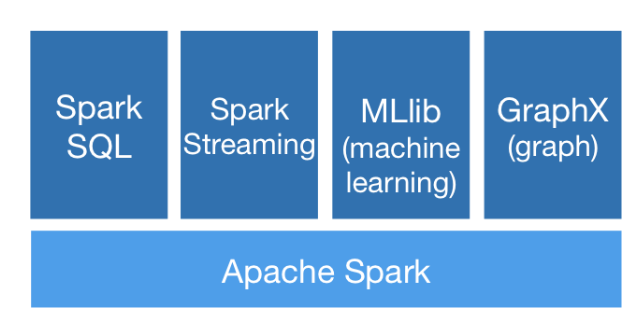
\includegraphics{Images/Spark.png}
    \caption{Spark modules}
    \label{fig:spark}
\end{figure}

\subsubsection{Spark-ML}
The Spark-ML library \cite{pysparkML} presents an API for simple machine learning implementations in Python. Spark-ML is the python variant of the Spark library MLlib. This is used for clustering of the street crime data points. The machine learning algorithms made available in this library take data frames as input and produce output in the form of data frames as well. This library contains many different classification and clustering machine learning algorithms such as naive bayes classifiers and k-means clustering. This project makes use of the bisecting k-means clustering algorithm. \\

\textbf{Bi-sectional K-Means Clustering}\\
Traditional k-means clustering requires the user to define a number of clusters to be created. Each observation from the data set is subsequently compared to each of the randomly chosen cluster centroids to determine which is closest. Closeness is calculated by the multi-dimensional distance between the values of each feature between two observations. After randomly selecting the cluster centroids every observation is assigned to a centroid. Once this is complete, the centers of the newly computed clusters replace the original centroids. This continues until the average distance from each observation to its centroid can no longer be decrease \cite{kMeans}. However, k-means clustering is prone to getting stuck in local minima points. In contrast, bi-sectional k-means clustering (BKM) is a variant developed to combat this weakness.

%What is BKM
BKM functions by randomly assigning initial cluster centroids after which k-means with a \textit{k} of two is continuously carried out on the cluster with the largest error until the desired number of clusters is achieved. Error is defined as the total distance from each observation to the centroid of its assigned cluster \cite{bkmGeneral}. BKM not only avoids local minima, but is generally more efficient than traditional k-means clustering for larger values of \textit{k}(number of clusters) due to the fact that only the data points of a single cluster are involved in the computation  \cite{bkmGood}.\\

\subsubsection{Spark-SQL}
Th Spark-SQL library \cite{pysparkSQL} is used for working with large data sets. Spark-SQL is the python variant of the Spark library Spark-SQL. This library allows these data sets to be read and written to HDFS while also containing the functionality to transform input to a format that the aforementioned machine learning library will accept (i.e. from CSV to data frame). 

\subsection{Drill}
Drill is a query engine that enables SQL queries to almost any data source. It is able to read from Hadoop, CSV-files, NoSQL data stores, cloud storage etc.  Drill combines speed with flexibility and is able to scale from a single laptop to a large cluster. Drill supports queries through a web interface, JDBC connections and a REST API. Drill gives the possibility to change between HDFS, no-SQL, SQL, local files and much more without ever having to change how the server fetches the data needed. This enables experimentation with different technologies and easier modifications to the setup. For this reason, Drill is useful as a query interface to the cluster environment. 


\end{document}